\chapter{Architettura del Software e Strutture Dati}
\label{cap:architettura}

\section{Organizzazione dei Moduli}

Il codice è un unico insieme di sorgenti C11 e assembly NASM, organizzato in moduli con responsabilità distinte (Figura~\ref{fig:architettura}). Le quattro varianti richieste dal corso non sono più quattro copie del programma, come nella versione d'esame, ma quattro compilazioni degli stessi sorgenti, prodotte dal \codice{Makefile} (Tabella~\ref{tab:varianti}): la precisione dipende dall'architettura di destinazione, attraverso il tipo \codice{real\_t} definito in \codice{common.h}, e OpenMP si attiva con l'opzione \codice{-fopenmp} del compilatore. Senza di essa le direttive \codice{\#pragma omp} vengono ignorate e il programma resta sequenziale.

\begin{figure}[H]
    \centering
    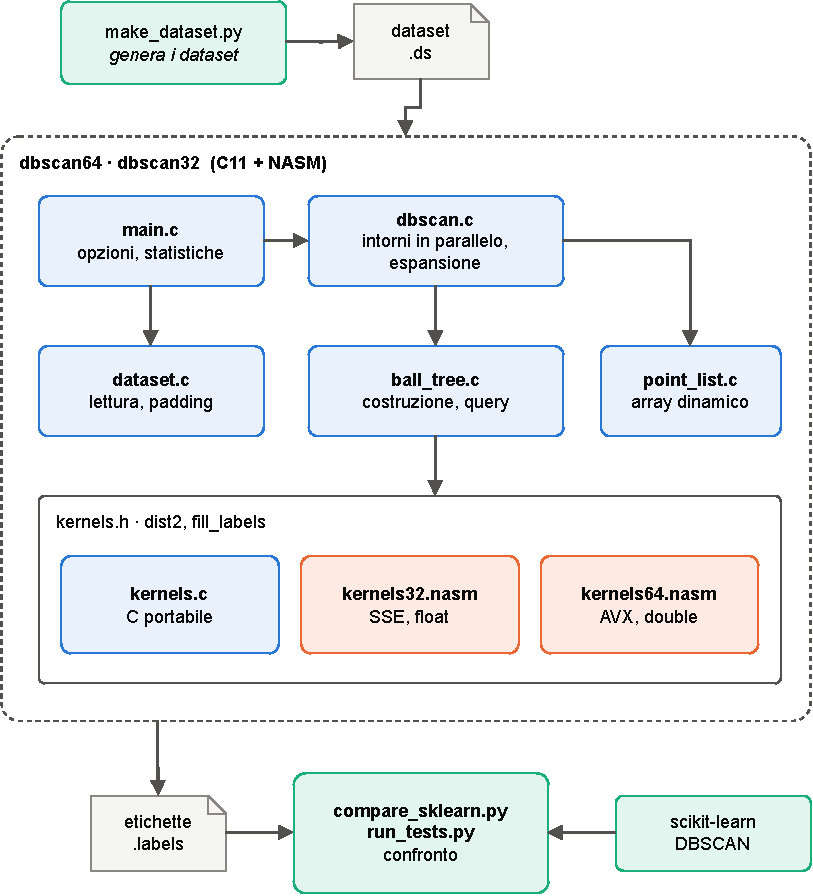
\includegraphics[width=0.85\textwidth]{diagrammi/architettura.pdf}
    \caption{Moduli del programma e strumenti di supporto. In blu i moduli C, in arancione i kernel assembly, in verde gli script Python.}
    \label{fig:architettura}
\end{figure}

\begin{table}[H]
    \centering
    \small
    \begin{tabular}{llll}
        \toprule
        \textbf{Eseguibile} & \textbf{Architettura} & \textbf{Precisione e kernel} & \textbf{OpenMP} \\
        \midrule
        \codice{dbscan32}     & x86-32 & \codice{float}, SSE  & no \\
        \codice{dbscan32-omp} & x86-32 & \codice{float}, SSE  & sì \\
        \codice{dbscan64}     & x86-64 & \codice{double}, AVX & no \\
        \codice{dbscan64-omp} & x86-64 & \codice{double}, AVX & sì \\
        \bottomrule
    \end{tabular}
    \caption{Le quattro varianti prodotte da \codice{make}.}
    \label{tab:varianti}
\end{table}

I moduli sono i seguenti:

\begin{itemize}
    \item \codice{main.c}: interpreta la riga di comando, carica il dataset, invoca l'algoritmo e stampa le statistiche, anche in formato JSON per gli script di misura;
    \item \codice{dataset.c}: legge i file, converte i valori in \codice{real\_t}, completa le righe con zeri e le allinea in memoria; scrive le etichette;
    \item \codice{dbscan.c}: l'algoritmo in due fasi della Sezione~\ref{sec:due-fasi} e la ricerca esaustiva;
    \item \codice{ball\_tree.c}: costruzione e interrogazione del Ball Tree;
    \item \codice{point\_list.c}: l'array dinamico di indici usato per gli intorni e come pila;
    \item \codice{kernels.h}: l'interfaccia dei due kernel, la distanza al quadrato \codice{dist2} e il riempimento delle etichette \codice{fill\_labels}, con una versione in C (\codice{kernels.c}) e una in assembly per ciascuna architettura (\codice{asm/kernels32.nasm} e \codice{asm/kernels64.nasm}). La versione da usare è scelta all'avvio tramite un puntatore a funzione, così che le due si possano confrontare con lo stesso eseguibile.
\end{itemize}

Accanto al programma, alcuni script Python completano il progetto:
\begin{itemize}
    \item \codice{make\_dataset.py} genera i dataset;
    \item \codice{compare\_sklearn.py} e \codice{tests/run\_tests.py} confrontano le etichette con quelle di scikit-learn;
    \item \codice{benchmark.py} esegue le misure del Capitolo~\ref{cap:sperimentazione}, e \codice{report\_data.py} ne ricava tabelle e grafici.
\end{itemize}

\section{Formato dei File e Disposizione in Memoria}

\subsection*{Formato dei file}

Il formato è quello del template del corso: due interi a 32 bit, il numero di colonne e il numero di righe, seguiti dai valori della matrice riga per riga (\emph{row-major order}). I valori sono numeri in virgola mobile a 32 o a 64 bit; il programma deduce la precisione dalla dimensione del file e converte i valori nel tipo della propria variante, così lo stesso dataset si può usare con entrambe le architetture. Le etichette sono scritte nello stesso formato, come matrice di una colonna di interi a 32 bit.

\subsection*{Padding e allineamento}
\label{sec:padding}

Le istruzioni SIMD lavorano su blocchi di quattro valori: quattro \codice{float} in un registro XMM a 128 bit o quattro \codice{double} in un registro YMM a 256 bit. Le istruzioni di caricamento allineato (\codice{movaps}, \codice{vmovapd}) richiedono inoltre che l'indirizzo sia multiplo della dimensione del registro, 16 o 32 byte, e generano un'eccezione in caso contrario. Il dataset viene quindi memorizzato come un unico blocco allineato, in cui ogni riga ha un numero di valori, detto \emph{stride}, pari alla dimensione $d$ arrotondata al multiplo di quattro successivo; le colonne aggiunte valgono zero e non alterano le distanze. Poiché la lunghezza di una riga in byte è un multiplo della dimensione di un registro, tutte le righe risultano allineate (Figura~\ref{fig:memoria}), e i kernel possono elaborare ogni riga a blocchi interi senza gestire un residuo.

\begin{figure}[H]
    \centering
    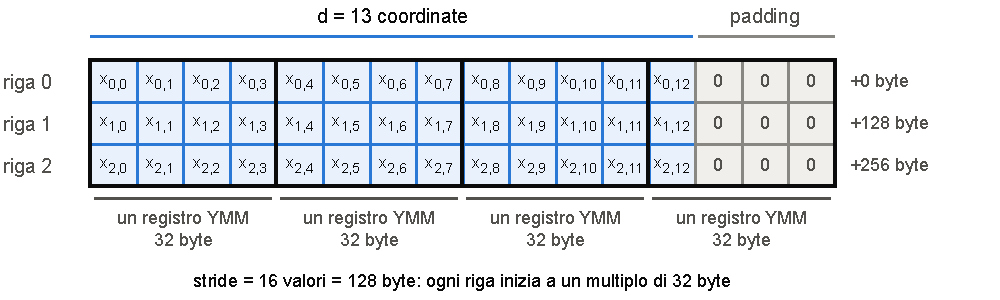
\includegraphics[width=\textwidth]{diagrammi/memoria.pdf}
    \caption{Disposizione in memoria di un dataset con $d = 13$ nella variante a 64 bit: ogni riga è completata con tre zeri fino a 16 valori, cioè 128 byte, e il blocco inizia a un indirizzo multiplo di 32.}
    \label{fig:memoria}
\end{figure}

La versione d'esame otteneva lo stesso risultato con la funzione \codice{adjust\_matrix}, che però allocava una seconda matrice senza liberare la prima; ora il completamento avviene durante la lettura, in un'unica allocazione.

\section{L'Array Dinamico PointList}

Gli intorni hanno dimensioni imprevedibili, da zero a $n-1$ punti. \codice{PointList} è un array di indici che raddoppia la propria capacità quando si riempie: il costo di un inserimento è costante in media, e la memoria sprecata è al più pari a quella usata. La stessa struttura serve da pila nella seconda fase.

Nella versione d'esame questo meccanismo, insieme alla deallocazione esplicita delle liste non più necessarie, era presentato come un sistema di \emph{garbage collection}; si tratta in realtà di gestione manuale della memoria con un array a crescita geometrica. Nella versione attuale ogni thread riusa la stessa \codice{PointList} per tutte le proprie interrogazioni, svuotandola di volta in volta, e copia il risultato in un vettore della dimensione esatta solo se il punto è core: le allocazioni si riducono a una per punto core.

\section{Il Ball Tree}

Un Ball Tree~\cite{omohundro1989} è un albero binario in cui ogni nodo rappresenta una ipersfera, detta \emph{ball}, che contiene un sottoinsieme dei punti: il centro è il centroide dei punti e il raggio è la distanza dal centro al punto più lontano. I due figli di un nodo si spartiscono i suoi punti; le foglie contengono al più \textit{leaf\_size} punti. Rispetto a un \emph{k-d tree}, che divide lo spazio con iperpiani paralleli agli assi, le sfere si adattano meglio alla distribuzione dei dati quando la dimensione cresce.

\begin{figure}[H]
    \centering
    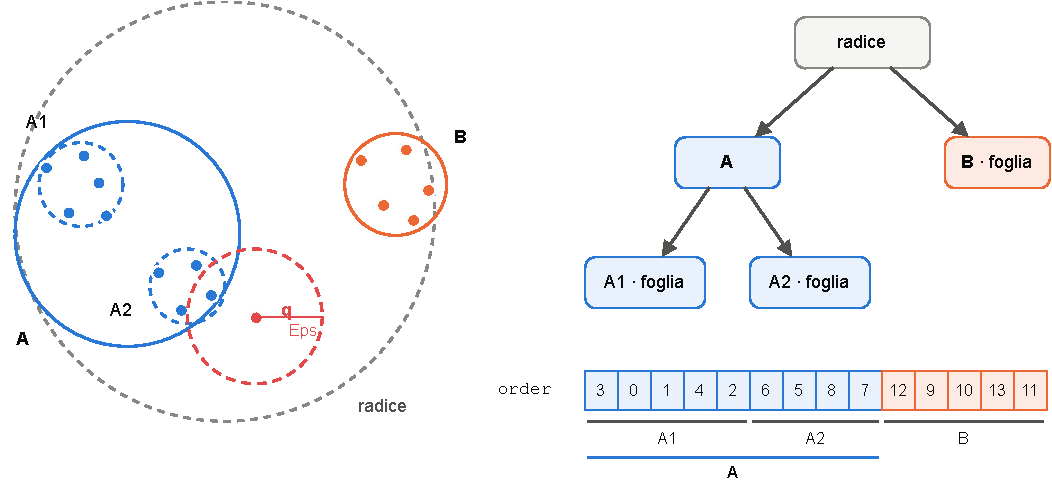
\includegraphics[width=\textwidth]{diagrammi/ball_tree.pdf}
    \caption{A sinistra, un Ball Tree su punti del piano: la radice contiene tutti i punti, i figli \textsf{A} e \textsf{B} ne contengono una parte ciascuno, \textsf{A} è divisa a sua volta in due foglie. L'intorno del punto $q$ interseca \textsf{A} e \textsf{A2}, mentre \textsf{B} viene esclusa senza calcolare alcuna distanza dai suoi punti. A destra, l'albero e il vettore \codice{order}, in cui ogni nodo occupa un intervallo contiguo.}
    \label{fig:balltree}
\end{figure}

\subsection*{Costruzione}

La costruzione parte da un nodo che contiene tutti i punti e lo divide ricorsivamente. Per dividere un nodo si scelgono due punti lontani tra loro: $p_1$, il più lontano dal centroide, e $p_2$, il più lontano da $p_1$. Ogni punto va poi con il più vicino dei due. Il criterio costa due scansioni lineari del nodo e tende a separare i gruppi di punti densi, perché $p_1$ e $p_2$ cadono agli estremi opposti della distribuzione.

L'albero non memorizza liste di punti per nodo. Tutti i nodi condividono un unico vettore di indici, \codice{order}, e la suddivisione ne riordina sul posto l'intervallo con uno schema a due indici simile a quello del \emph{quicksort}: ogni nodo occupa un intervallo contiguo \codice{[start, end)} di \codice{order}, i figli ne occupano le due metà (Figura~\ref{fig:balltree}). Nella versione d'esame ogni nodo allocava invece due nuove liste di punti e liberava quella del padre, con un gran numero di allocazioni. Al termine della costruzione le righe del dataset vengono copiate nell'ordine di \codice{order}: così la scansione di una foglia legge memoria contigua invece di saltare tra righe sparse. La copia raddoppia la memoria occupata dal dataset ma riduce il tempo di esecuzione del 20--40\%, come emerso durante lo sviluppo.

Un nodo diventa foglia quando ha al più \textit{leaf\_size} punti oppure quando tutti i suoi punti coincidono, perché in quel caso il raggio è nullo e nessuna divisione è possibile. La versione d'esame non gestiva questo caso: con più di \textit{leaf\_size} punti identici, tutti finivano nello stesso figlio e la ricorsione non terminava. È presente anche una salvaguardia per il caso, dovuto soltanto agli arrotondamenti, in cui uno dei due figli risulti vuoto.

\subsection*{Interrogazione}

Per trovare l'intorno di un punto $x$ si visita l'albero dalla radice. Per ogni nodo di centro $c$ e raggio $r$ si calcola $\delta = \mathrm{dist}(x, c)$ e, per la disuguaglianza triangolare, si distinguono tre casi:

\begin{enumerate}
    \item se $\delta > r + \varepsilon$, la sfera del nodo e l'intorno di $x$ sono disgiunti: il nodo e tutto il suo sottoalbero vengono esclusi;
    \item se $\delta + r \le \varepsilon$, la sfera è interamente contenuta nell'intorno: tutti i punti del nodo vengono accettati senza calcolarne le distanze;
    \item altrimenti si prosegue sui figli, oppure, in una foglia, si calcola la distanza di ogni punto.
\end{enumerate}

Il secondo caso non era presente nella versione d'esame ed è decisivo quando $\varepsilon$ è grande rispetto alla scala dei dati, come nel dataset usato per l'esame: la Sezione~\ref{sec:caso-esame} mostra che riduce le distanze calcolate da 25 milioni a circa cinquemila. Le distanze dai centri sono le uniche per cui si estrae la radice quadrata, perché i test confrontano somme di distanze; i centroidi sono allocati allineati e completati come le righe del dataset, quindi anche queste distanze usano i kernel SIMD.

\section{Interfaccia a Riga di Comando}

La Tabella~\ref{tab:opzioni} riassume le opzioni del programma. Rispetto al template sono state eliminate le opzioni \codice{-k} e \codice{-labels}, ereditate da un altro progetto del corso e ignorate dall'algoritmo, e sono state aggiunte quelle che selezionano l'indice, i kernel e il numero di thread: le varianti confrontate nel Capitolo~\ref{cap:sperimentazione} si ottengono tutte dallo stesso eseguibile, senza modificare il codice.

\begin{table}[H]
    \centering
    \small
    \begin{tabularx}{\textwidth}{lX}
        \toprule
        \textbf{Opzione} & \textbf{Significato} \\
        \midrule
        \codice{-i}, \codice{--input FILE} & dataset da elaborare \\
        \codice{-e}, \codice{--eps EPS} & raggio $\varepsilon$ dell'intorno \\
        \codice{-m}, \codice{--min-pts N} & soglia \textit{MinPts}, punto stesso incluso \\
        \codice{-o}, \codice{--output FILE} & file in cui scrivere le etichette \\
        \codice{--index KIND} & \codice{balltree} (predefinito) oppure \codice{linear}, la ricerca esaustiva \\
        \codice{--leaf-size N} & punti massimi in una foglia del Ball Tree (predefinito 32) \\
        \codice{--no-simd} & usa i kernel in C invece di quelli SSE/AVX \\
        \codice{-t}, \codice{--threads N} & numero di thread OpenMP (predefinito: tutti i core logici) \\
        \codice{--json} & stampa risultati e tempi come una riga JSON \\
        \codice{-q}, \codice{--quiet} & non stampa nulla oltre agli errori e alla riga JSON \\
        \bottomrule
    \end{tabularx}
    \caption{Opzioni della riga di comando.}
    \label{tab:opzioni}
\end{table}
